\documentclass[10pt]{article}
\usepackage{setspace}
\usepackage{amsmath,amssymb}
\usepackage{amsthm}
\usepackage{fancybox}
\usepackage{algorithm, algpseudocode}
\usepackage{url}



\usepackage{enumitem}
\usepackage{multirow}
\usepackage{color}
\usepackage{graphicx}
\usepackage{setspace}
\usepackage{comment}
\usepackage{bm}

\begingroup
\renewcommand{\section}[2]{}%
%\renewcommand{\chapter}[2]{}% for othe

\newcommand*{\KeepStyleUnderBrace}[1]{%f
  \mathop{%
    \mathchoice
    {\underbrace{\displaystyle#1}}%
    {\underbrace{\textstyle#1}}%
    {\underbrace{\scriptstyle#1}}%
    {\underbrace{\scriptscriptstyle#1}}%
  }\limits
}

\usepackage{wrapfig}
\usepackage[margin=0.7in]{geometry}
 
\allowdisplaybreaks[4]
\usepackage{bbm}


\usepackage{amsrefs}
\usepackage{mathtools}
\mathtoolsset{showonlyrefs=true}


\usepackage[utf8]{inputenc}
\usepackage{hyperref}
\hypersetup{
    colorlinks=true,
    citecolor = blue,
    linkcolor=blue,
    filecolor=magenta,           
    urlcolor=cyan,
}

\usepackage[breakable, theorems, skins]{tcolorbox}
\DeclareRobustCommand{\mybox}[2][gray!20]{%
\begin{tcolorbox}[   %% Adjust the following parameters at will.
        breakable,
        left=0pt,
        right=0pt,
        top=0pt,
        bottom=0pt,
        colback=#1,
        colframe=#1,
        width=\dimexpr\textwidth\relax, 
        enlarge left by=0mm,
        boxsep=5pt,
        arc=0pt,outer arc=0pt,
        ]
        #2
\end{tcolorbox}
}


\theoremstyle{plain}
\newtheorem{thm}{Theorem}

\theoremstyle{definition}
\newtheorem{open}[]{Open problems}

 \usepackage[parfill]{parskip}
 
\usepackage[font=scriptsize,labelfont=bf]{caption}

\input macros.tex

\begin{document}

\begin{doublespace}

{\bf Title}: The Good, the Bad, the Pragmatic: Tensor Methods for Network Learning \\

{\bf Author}: Dr. Miaoyan Wang, Assistant Professor in Department of Statistics, Affiliated with Institute for the Foundations of Data Science (IFDS)\\

{\bf WISPER Record Number}: MSN251318\\

{\bf Abstract}: The prevailing theme in the proposal is to develop powerful tensor methods for high-dimensional multi-layer network analysis. Rapid developments in modern technologies have made large-scale network datasets readily available. Modern networks are not only large in size, but they also have intricate structure. It is therefore of great importance to find a low-dimensional representation to better understand the key structure buried in noisy observations. 

Higher-order tensors provide effective representation of multi-layer networks using multi-way structure. The PI will develop a framework --- of tensor models, efficient algorithms, and softwares --- to analyze multi-layer networks. Previous literature has advocated unfolding the tensor into a matrix and applying classical methods developed for matrices. Despite the popularity of such techniques, tensor method provides more powerful tools to capture complex structures in data that lower-order methods fail to exploit. The research goal goes beyond the traditional multivariate analysis; we aim to characterize probabilistic distributions over multi-layer edge connections, while taking into accounting the higher-order structures such as transitivity, balance, and community. This will allow researchers to examine complex interactions among entities in a context-specific manner, thereby providing solutions to questions that were previously impossible. The software packages resulting from this proposal, will be released freely, as well as related visualization tools for network analyses.
\end{doublespace}
\newpage

\begin{center}
\vspace{.2cm}
{\bf \large The Good, the Bad, the Pragmatic: Tensor Methods for Network Learning }\\
\end{center}
\vspace{.2cm}

My research project is broadly driven by questions related to understanding hidden salient structures of complex network datasets. The questions and techniques that we develop span across the fields of information theory, machine learning, and quantitative social sciences. 

{\bf Motivations.} A central theme in modern data analysis is to find a low-dimensional representation to better understand, compress, and convey the key phenomena buried in noisy observations. Modern datasets are not only large in size, but they also have intricate structure. A typical example is in the form of {\bf network}~\cite{bickel2009nonparametric,rohe2011spectra,zheng2019}, which is quantitative representation of interactions between entities in complex systems. As real-world networks are huge in nature, dimension deduction is crucial for pattern detection and subsequent specialized tasks. 

In network studies, researcher are interested in interpretable low-dimensional structure within the high-dimensional relational data. The question goes beyond the traditional multivariate analysis; we aim to characterize probabilistic distributions over pairwise edge connections, while taking into accounting the higher-order structures such as transitivity (``a friend of a friend is a friend''), balance (``an enemy of a friend and an enemy''), and community (``cohesive subgroups of nodes''). {\bf My project targets at developing higher-order tensor methods for analyzing high-dimensional network data.} The resulting prototypes will facilitate automatic detection of hidden salient structure in network data, thereby providing solutions to questions that cannot be addressed by existing methods. I will elaborate two specific directions for social network learning using tensor methods. 

{\bf Community detection in multi-layer networks.}
A multi-layer network consists of multiple undirected graphs (or adjacency matrices), where each graph represents the connection among the same set of vertices (Fig~\ref{fig:1}a-b). The dataset is naturally organized as an order-3 tensor with the first two modes being vertices and the third mode being the contexts under which the graph is observed. Multilayer networks arise commonly in longitudinal study and multi-relational analysis. While the community structure in each single-layer network has been widely analyzed in the literature, little work has studied the heterogeneous pattern across multiple layers. 

\begin{figure}[H]
\vspace{-.2cm}
\begin{center}
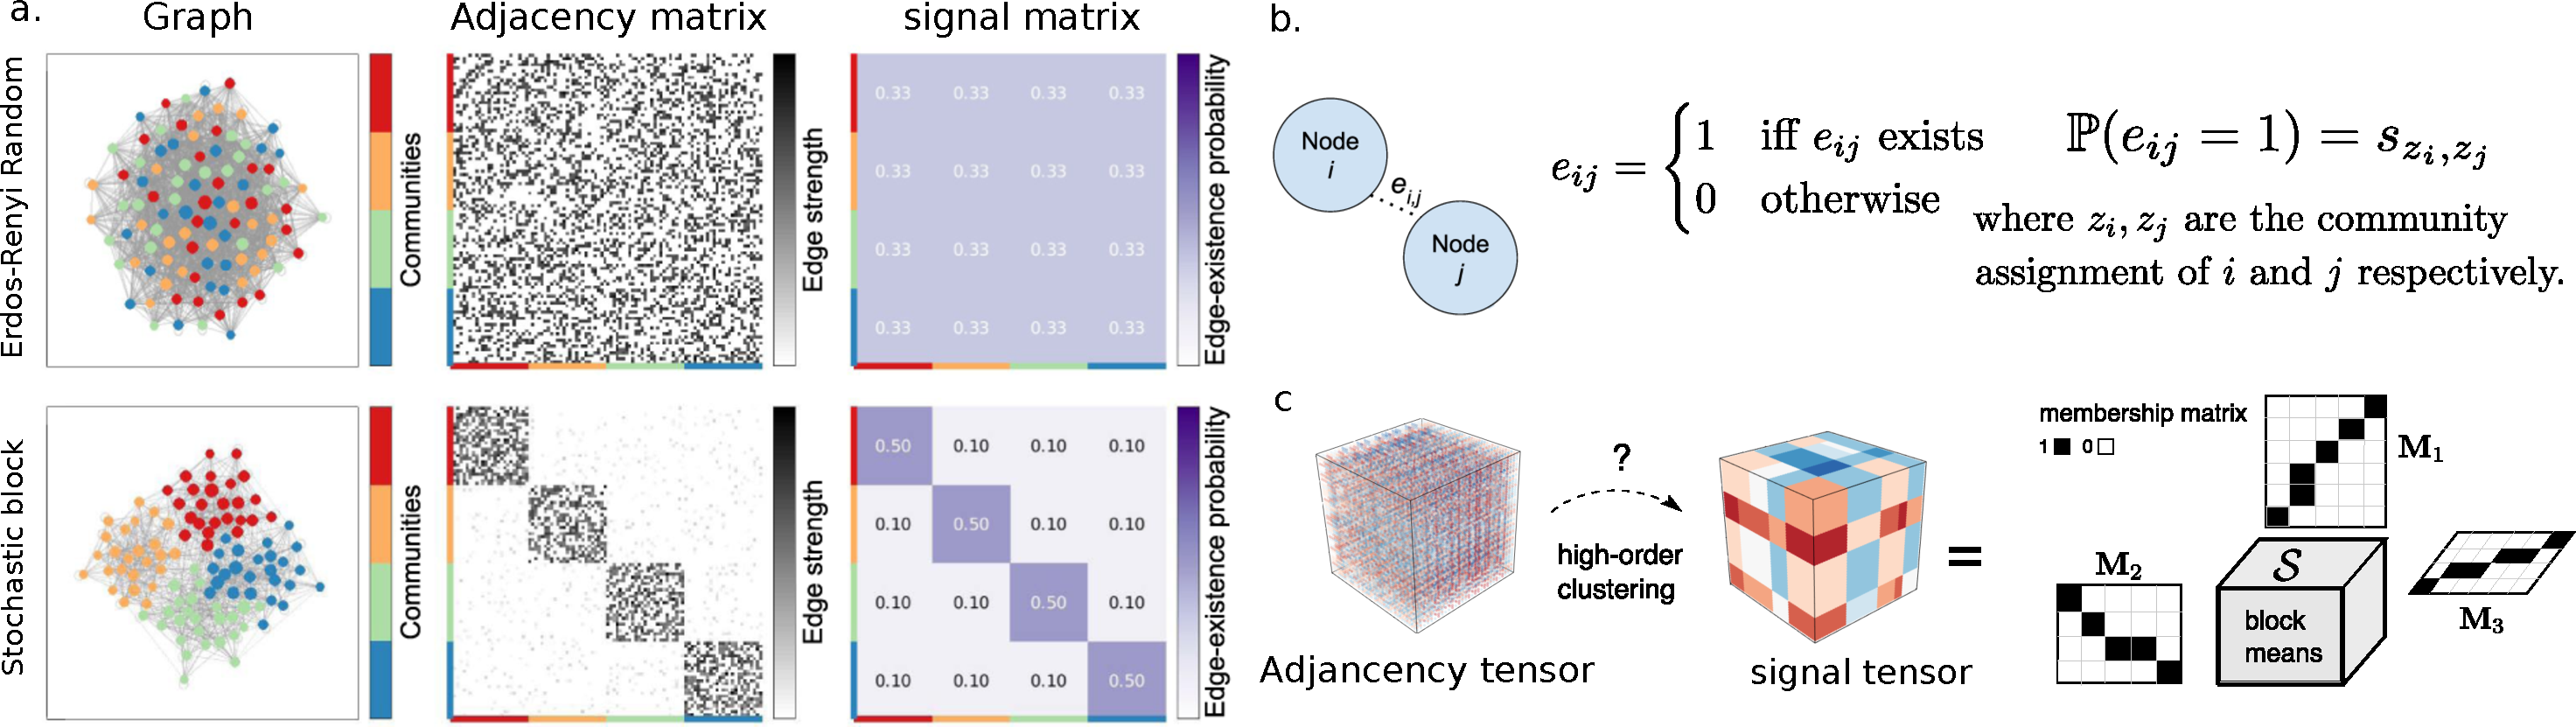
\includegraphics[width=.9\textwidth]{network1.pdf}
\caption{(a) Representation of network data using adjacency matrices~\cite{faskowitz2018weighted}. (b) Stochastic block model for single-layer network (i.e., matrix). (c) We propose tensor extension of block model for high-order clustering in the context of multi-layer networks~\cite{hu2019generalized,han2020exact}.}\label{fig:1}
\end{center}
\vspace{-.6cm}
\end{figure}

Methods built on tensors provide generalized tools to capture complex data structure that the off-the-shelf methods may fail to exploit. We develop a tensor stochastic block model~\cite{wang2019multiway,han2020exact} for simultaneous clustering of entities along each mode. 
\begin{wrapfigure}{r}{.41\linewidth}
  \vspace{-.3cm}
  \begin{center}
    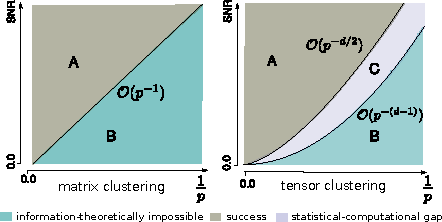
\includegraphics[width=.4\textwidth]{demo_snr.pdf}
  \end{center}
          \vspace{-.2cm}
    \caption{\scriptsize Comparison between matrix and tensor methods.}\label{fig:2}
        \vspace{-.4cm}
\end{wrapfigure} 
Specifically, let $\tZ=\entry{z_{i_1,\ldots,i_d}}\in\{0,1\}^{p\times \cdots \times p}$ denote the order-$d$ adjacency data tensor, where the entries $z_{i_1,\ldots,i_d}$ represent the presence or absence of edge $(i_1,i_2)$ at context $(i_3,\ldots,i_d)$. We model the signal tensor $\mathbb{E}(\tZ)$ using block structure
\[
\mathbb{E}(\tZ)=\tS\times_1\mM_1\times_2\cdots \times_d\mM_d,
\]
for some low-dimensional core tensor $\tS$ and community membership matrices $\mM_1,\ldots,\mM_d$ (see Figure~\ref{fig:1}c). The learning goal is to estimate $d$-way connection strength tensor $\tS$ and community assignment $(\mM_1,\ldots,\mM_d)$ from a noisy observation $\tZ$. We propose a higher-order Lloyd algorithm, which uses alternating optimization for parameter estimations. Our preliminary analysis shows that the tensor algorithm achieves \emph{exact recovery of communities} under less stringent assumptions than existing algorithms. Surprisingly, we find that the learning performance is fully characterized by signal-to-noise ration (SNR) (see Figure~\ref{fig:2}). In the strong SNR region A, we prove that the our algorithm achieves exact clustering \emph{in polynomial time}. We also show that the estimation error bound of the target tensor is \emph{free of tensor dimension}. This feature is especially appealing in modern large-scale network analysis. In the weak SNR region B, we provide evidence to the conjecture of information-theoretical impossibility of consistent clustering. In the modest SNR region C, the problem exhibits a gap between computational and statistical limits, a phenomenon that has drawn much interests in modern learning problems~\cite{berthet2013complexity,brennan2018reducibility,wu202113}. Our result provides the first characterization of trade-off for higher-order clustering, and the established results serve the benchmark for algorithm development. 


{\bf Learning latent patterns in network.} 
When analyzing imaging data, one can learn individual patches and pixels (local features) or total variations (global feature) in order to extract useful information from images (Figure~\ref{fig:3}a). Analogously for networks, one may learn their local structures (e.g., nodes and edges) or global structure (community or core-periphery structures). At the same time, we are facing ever-growing network size due to the explosion of recent technology in measuring, processing, and storing network data. Hence, it would be an important and timely contribution to develop algorithms that compress a large network into a set of multi-scale, interpretable structures.

\begin{figure}[H]
\begin{center}
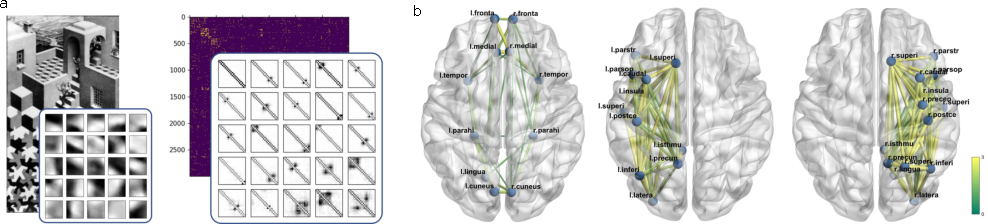
\includegraphics[width=1\textwidth]{example_new.pdf}
\caption{(a) Latent motifs learned from images and social network data~\cite{lyu2020online}. (b) Connectivity motifs learned from human brain networks~\cite{lee2020tensor}. }\label{fig:3}
\end{center}
\end{figure} 
\vspace{-.4cm}

We propose to develop a systematic approach to learning latent \emph{network motifs} that form the salient architecture of networks. Our method is based on structured tensor decomposition where each rank-1 tensor is interpreted as a latent motif for multi-way interaction. The ability to encode a network using a set of latent motifs opens up a wide variety of network-analysis tasks, such as network completion, denoising, and link prediction. For example, Figure~\ref{fig:3}a shows 25 latent motifs learned from images and social network data based on nonnegative matrix decomposition. My group has been generalizing the method to tensors and applying the method to Human Connectome Project (HCP). The result reveals a clear spatial separation among brain node between hemispheres (Figure~\ref{fig:3}b). The identified latent similarities among nodes \emph{without external labels} highlights the potential power of tensor methods to pattern discovery. 

The latent motif learning is challenging because of the extremely high dimensionality in the network data. The PI's previous extensive experience on tensor related work has shown that tensors sought in network applications often possess special structures, such as low-rankness~\cite{wang2017operator,wang2020learning,lee2021beyond}, sparsity~\cite{wang2018two}, non-negativity~\cite{wang2019three}, or orthogonality~\cite{wang2017tensor}. We will leverage the formalisms of \emph{intrinsic dimension} to develop efficient statistical methods for analyzing these high-dimensional datasets. We will further develop adaptive, semi-supervised methods that incorporate practical constraints, such as incomplete observation, corrupted distributions, and computation with time and memory constraints. 

%\mybox[gray!20]{{\bf Impact and Significance:} 
%\begin{itemize}[leftmargin=*]
%\item Develop efficient prediction tools for tensor classification, tensor regression, and deep tensor neural network in the presence of domain constraints.
%\item Build data-driven prototypes that integrate machine learning into the multi-modal signal integration.
%\end{itemize}
%}

%{\bf  Phase transition in clustering within higher-order tensor data.} High-order tensors have received increasing recent attention in enormous fields including social networks, computer vision, neuroscience, and genomics. Tensors provide effective representation of the hidden structure in multiway data. One of the popular structure utilized in tensor data analysis is the so-called low-rankness. An order-d tensor $\tX$ is called Tucker low-rank if it can be decomposed as a tensor-matrix product 
%\[
%\tX=\tS\times_1\mM_1\times \cdots \times_d\mM_d
%\]
%for some low-dimensional core tensor $\tS$ and loading matrices $\mM_1,\ldots,\mM_d$.

%\mybox[gray!20]{
%{\bf Impact and Significance:} 
%\begin{itemize}[leftmargin=*]
%\item Develop interactive data exploration and visualization for learning with complex network data. 
%\item Design robust tools to analyze tensor data and to detect community patterns for recommendation system applications. 
%\end{itemize}
% }

{\bf Deliverables and Milestones.}
The PI is a young faculty in statistics with affiliation in Institute for the Foundations of Data Science (IFDS). The PI has actively contributed to several multi-institutional consortiums, in collaboration with researchers in both academics and industry. This grant will support the PI's group to further create a diverse working group. Open-source software will be released, as the fruit of the research, that facilitates academia, industry, and society to analyze complicated tensor data.  The following table summarizes the planned milestones. 
\vspace{-.3cm}
\begin{center}
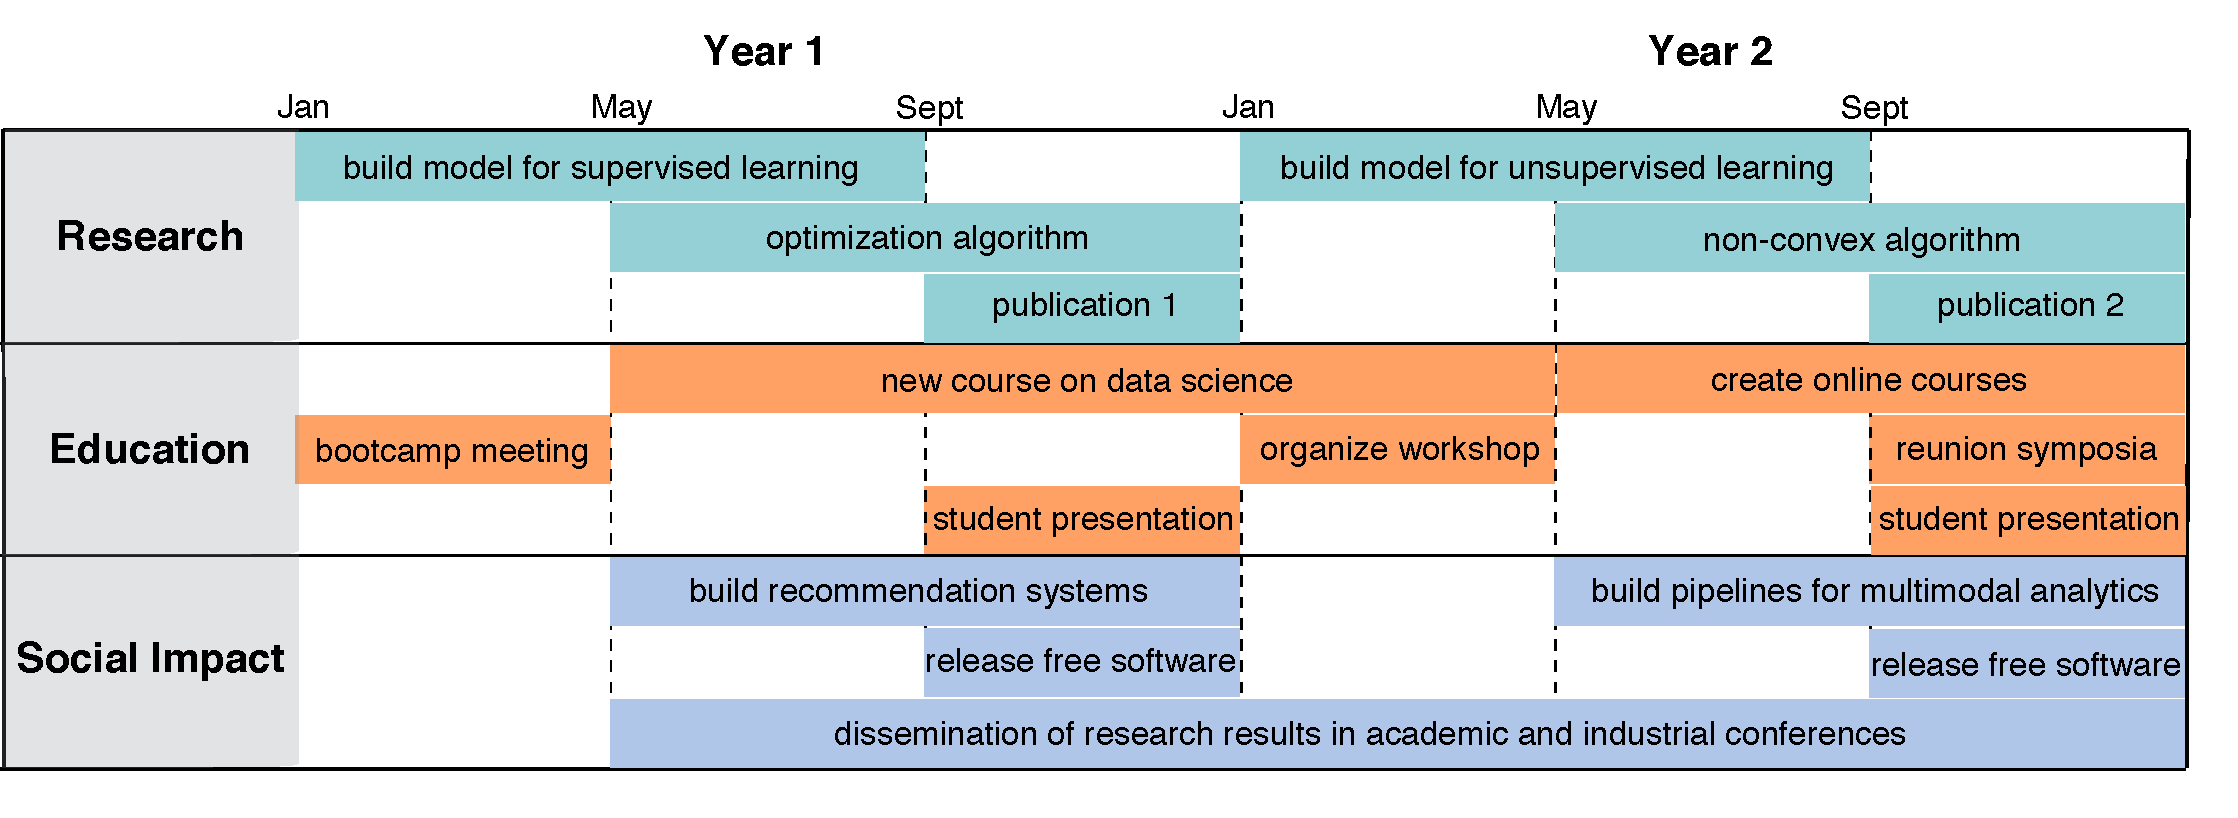
\includegraphics[width=.9\textwidth]{milestone.pdf}
\end{center}
\vspace{-.4cm}
%The project will create deliverables in three aspects: {\bf Research}, {\bf Education}, and {\bf Social impact}. I plan to devote one year for each of the aforementioned research problems. Regarding teaching, I will create a new course on \emph{data science} in both traditional and online formats. The new course will introduce students to the real word challenges in implementing statistical machine learning approaches to decision making. Open-source software will be released, as the fruit of the research, that facilitates academia, industry, and society to analyze complicated tensor data. The PI will organize a series of workshops on the scientific applications of tensor data analysis, with the aim to encourage interdisciplinary collaborations. 

\newpage
\vspace{1cm}
{\bf \large References}
{ \large 
\begin{thebibliography}{9}
\bibitem{berthet2013complexity} 
Quentin Berthet and Philippe Rigollet, Complexity theoretic lower bounds for sparse principal component detection, \emph{Conference on learning theory (COLT)}, 2013, pp. 1046–1066.
\bibitem{bickel2009nonparametric}
Peter J Bickel and Aiyou Chen, A nonparametric view of network models and Newman–Girvan and other modularities, \emph{Proceedings of the National Academy of Sciences (PNAS)} 106 (2009), no. 50, 21068–21073.
\bibitem{brennan2018reducibility}
Matthew Brennan, Guy Bresler, and Wasim Huleihel, Reducibility and computational lower bounds for problems with planted sparse structure, \emph{Conference on learning theory (COLT)}, 2018, pp. 48–166.
\bibitem{faskowitz2018weighted}
Joshua Faskowitz, Xiaoran Yan, Xi-Nian Zuo, and Olaf Sporns, Weighted stochastic block models of the human connectome across the life span, \emph{Scientific reports} 8 (2018), no. 1, 1–16.
\bibitem{hu2019generalized}
Jiaxin Hu, Chanwoo Lee, and {\bf Wang, Miaoyan},  Supervised tensor decomposition with interactive side information, Advances in \emph{Neural Information Processing Systems (NeurIPS)} 33 Workshop on Machine Learning and the Physical Sciences, 2020.

This work wins {\bf Best Student Paper Award} from the Statistical Computing and Graphics Section of American Statistical Association (ASA), 2021.

\bibitem{han2020exact}
Rungang Han, Yuetian Luo, {\bf Miaoyan Wang}, and Anru R Zhang, Exact clustering in tensor block model: Statistical optimality and computational limit, arXiv preprint arXiv:2012.09996 (2020). 

This work wins {\bf Best Student Paper Award} from the Statistical Learning and Data Science Section of the American Statistical Association (ASA), 2021.

\bibitem{lee2020tensor}
Chanwoo Lee and {\bf Miaoyan Wang}, Tensor denoising and completion based on ordinal observations, \emph{International conference on machine learning (ICML)}, 2020, pp. 5778–5788.
\bibitem{lee2021beyond}
Chanwoo Lee and {\bf Miaoyan Wang}, Beyond the signs: Nonparametric tensor completion via sign series, arXiv preprint arXiv:2102.00384 (2021).
\bibitem{lyu2020online}
Hanbaek Lyu, Deanna Needell, and Laura Balzano, Online matrix factorization for markovian data and applications to network
dictionary learning, \emph{Journal of Machine Learning Research} 21 (2020), no. 251, 1–49.

\bibitem{rohe2011spectra}
Karl Rohe, Sourav Chatterjee, and Bin Yu. Spectral clustering and the high-dimensional stochastic blockmodel.  \emph{Annals of Statistics}, Vol 39, 4, 1878--1915, 2011. 

\bibitem{wang2017operator}
{\bf Miaoyan Wang}, Khanh Dao Duc, Jonathan Fischer, and Yun S Song, Operator norm inequalities between tensor unfoldings on the partition lattice, \emph{Linear Algebra and Its Applications} 520 (2017), 44–66.
\bibitem{wang2019three}
{\bf Miaoyan Wang}, Jonathan Fischer, and Yun S Song, Three-way clustering of multi-tissue multi-individual gene expression data using semi-nonnegative tensor decomposition, \emph{The Annals of Applied Statistics} 13 (2019), no. 2, 1103–1127.
\bibitem{wang2020learning}
{\bf Miaoyan Wang} and Lexin Li, Learning from binary multiway data: Probabilistic tensor decomposition and its statistical optimality, \emph{Journal of Machine Learning Research} 21 (2020), no. 154, 1–38.
\bibitem{wang2018two}
{\bf Miaoyan Wang}, Fabrice Roux, Claudia Bartoli, Carine Huard-Chauveau, Christopher Meyer, Hana Lee, Dominique Roby, Mary Sara McPeek, and Joy Bergelson, Two-way Mixed-effects methods for joint association analysis using both host and pathogen genomes, \emph{Proceedings of the National Academy of Sciences (PNAS)} 115 (2018), no. 24, E5440–E5449.
\bibitem{wangstrategy}
{\bf Miaoyan Wang}, Johanna Jakobsdottir, Albert V. Smith, and Mary Sara McPeek. G-STRATEGY: Optimal selection of individuals for sequencing in genetic association studies. \emph{Genetic Epidemiology}, Vol. 40, No. 6, 446–460, 2016.

Highlighted as {\bf Editor's Pick Paper} of this issue. This work wins {\bf  ASHG Charles J. Epstein Trainee Award} and {\bf  IGES Williams Award}. 
\bibitem{wang2017tensor}
{\bf Miaoyan Wang} and Yun Song, Tensor decompositions via two-mode higher-order SVD (HOSVD), \emph{Artificial intelligence and statistics}, 2017, pp. 614–622.
\bibitem{wang2019multiway}
{\bf Miaoyan Wang} and Yuchen Zeng, Multiway clustering via tensor block models, \emph{ Advances in Neural Information Processing Systems (NeurIPS)} 32 . (2019).
\bibitem{wu202113}
Yihong Wu and Jiaming Xu, Statistical problems with planted structures: Information-theoretical and computational limits, \emph{Information-Theoretic Methods in Data Science} (2021), 383.

\bibitem{zheng2019}
L Zheng and G Raskutti. Testing for high-dimensional network parameters in auto-regressive models. \emph{Electronic Journal of Statistics}, 13(2): 4977-5043 (2019). 

\end{thebibliography}
}

%\bibliography{tensor_wang}
%\bibliographystyle{plain}
\end{document}